\documentclass[letterpaper, 11pt]{article}%can be jou (for journal), man (manuscript) or doc (document)
%these next packages extend the apa class to allow for including statistical and graphic commands
\usepackage{hyperref}   %this allows us to cite URLs in the text
\usepackage[protrusion=true,expansion=true]{microtype} % Better typography
\usepackage{graphicx}  %allows for graphic to float when doing jou or doc style
\usepackage{amssymb}  %use formatting tools  for math symbols
% type setting of functions, packages, and R follows a particular style
\usepackage{mathpazo} % Use the Palatino font
% \usepackage{apacite}
\usepackage{siunitx}
\usepackage{graphics}
\usepackage{textcomp}
\usepackage{gensymb}
\usepackage{multirow}
\usepackage{float}
\usepackage[nottoc]{tocbibind}
\usepackage[font=footnotesize, labelfont=bf]{caption}
% \usepackage[numbers]{natbib}
\usepackage[T1]{fontenc} % Required for accented characters
\linespread{2.0} % Change line spacing here, Palatino benefits from a slight increase by default
\let\proglang=\textsf
\newcommand{\R}{\proglang{R}}
\newcommand{\pkg}[1]{{\normalfont\fontseries{b}\selectfont #1}}
\newcommand{\Rfunction}[1]{{\texttt{#1}}}
\newcommand{\fun}[1]{{\texttt{#1}}}
\newcommand{\Robject}[1]{{\texttt{#1}}}
\newcommand{\at}{\makeatletter @\makeatother}
% \raggedbottom
%
%
%Here is where we start the important APA stuff
\begin{document}

\title{\textbf{CMPT 318 Final Project}}
\author{R. Matheson Mawhinney - 301194286 \\ Alexis Lizardo - 301318503 \\ Truong Thinh Nguyen - 301215714}

\maketitle
% \newpage

\abstract{Infrastructure such as the water supply and power grids are prime targets for cyber attackers, and as such it is of critical importance to keep them safe. Sadly, providing perfect protection is not possible. Instead, systems must be developed to detect attacks quickly to mitigate damage. This paper will describe the implementation and results of such a system, using hidden Markov Models to detect anomalous data within datasets taken from a power grid. Furthermore, it will discuss the benefits of using this system, and how it can be improved further in the future.}

\newpage
\tableofcontents
\newpage
\listoffigures
\newpage

\section{Introduction}
  As more information is created in digital form and networks containing this information continue to grow, the threat of cyberattacks greatly increases. More troubling, is how these attacks are becoming increasingly complex and sophisticated, with attackers able to infiltrate systems and lie dormant, gathering information and learning about the system until they strike. While it is concerning to have these types of attacks happen to corporations, the threat of attack against vital infrastructure is of much greater concern. One such vital system is the power grid, which most of modern society relies on for even the most mundane of tasks.

This paper will illustrate a method of detecting attacks against such a system, using the concept of anomaly detection, to track down potential intruders in the system. Using Hidden Markov Models, it is possible to train a model with normal behaviour so that it can detect when usage outside of the norm has occurred. The goal of this method is to be able to detect suspicious behaviour within the power grid so that measures can be taken to investigate the oddities found, thereby preventing major attacks against critical infrastructure.


\section{Background}
Anomaly detection in the field of statistics is a well studied field with numerous different methods of finding outliers. The basic principle is to study a dataset in order to determine what the normal or expected behaviour of the data should be. Armed with that knowledge, various different techniques can be applied to the data to find data points that do not match the previously determined expectations.

\subsection{Anomalies}
In general, there are three different types of anomalies \cite{zahra}. The first is known as a point anomaly. A point anomaly is a single data point that falls outside the expected range of the surrounding data. What this range is, depends on what was previously defined as being expected. Secondly, there are contextual anomalies. Contextual anomalies are data points that may be normal and expected at one point in the dataset, but anomalous during another. For example, if measuring temperature over time, it might make sense for the temperature in the summer to be $25 \degree C$ at 12PM and $10 \degree C$ at 12AM. If we see a data point that falls to $10 \degree C$ at 12PM, we should consider it to be an anomaly. Finally, we have collective anomalies. Collective anomalies are anomalies that encompass a sequence of data points taken together. For example, in a computer, certain system calls may be called during its usage that are normal and expected. However, if a sequence of these calls happens in a specific order, it could signal that an attacker has attacked the computer\cite{chandola}.

\subsection{Markov Models}
One method for finding anomalies is by using Hidden Markov Models, or HMMs. In order to understand what a HMM is, it is important to first understand what the Markov Process is. The Markov Process states that the future state of a system is independent of the past, given the present, meaning that the next state the system transitions to depends only on the state that we are currently in, and nothing else. A Markov Model is a model that follows the Markov Process.

\begin{figure}
  \centering
  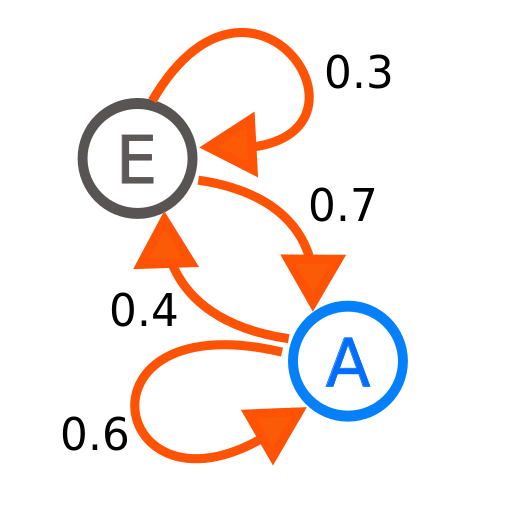
\includegraphics[scale=0.2]{process}
  \caption[Markov Process]
  {An example of the Markov Process \cite{markov}. Moving from state E to state A depends only on the probability given along the arrow from E to A and nothing else. }
\end{figure}

A Hidden Markov Model is very similar to a regular Markov Model in that they both have states and transition between those states following the Markov Process. In an HMM however, the states are not visible to the observer. Instead, the observer only sees the outcome of being in one of the states. As a result, the observer can see a sequence of outcomes, but cannot know in which order the model transitioned through the states to generate those outcomes.
Defining a HMM requires defining a few parameters \cite{Rabiner}:
\begin{enumerate}
  \item
  N, the number of states in the model
  \item
  M, the number of distinct observation symbols per state
  \item
  A, the matrix of transition probabilities
  \item
  B, the set of observation probabilities
  \item
  $\pi$, the initial state
\end{enumerate}
In general, an HMM can be defined using the tuple, $\lambda$ = (A, B, $\pi$) where A is the transition matrix, B is the outcome probabilities, and $\pi$ is the initial state.

While HMMs do a sufficient job of describing and modelling many systems, there are times when it is not specific enough. In these instances, another model, namely a Hidden Semi-Markov Model, can be used instead. An HSMM is very similar to an HMM, however the probability of transitioning depends on the amount of time the system has been in the current state. A simple example would be tracking a person's sleep/wake cycle. When a person goes to sleep, it is unlikely they will wake up soon. However, as time passes, it becomes more and more likely that their state will transition from sleeping to awake. HSMMs are harder to model than regular HMMs as the algorithms typically used to optimize an HMM are not designed to take time into account and must first be modified.

\subsection{The Power Grid}
Today's society is heavily reliant on electricity, and as such, the power grid has become one of the most critical infrastructures. Unfortunately, this has led to it becoming at risk of cyberattacks by foreign actors wishing to disrupt a nation's ability to function. While it may seem far-fetched for such an attack to occur, the reality is that it has already happened. On December 23, 2015 Ukraine's power grid was almost entirely crippled for up to six hours after being hit by a cyberattack, with Russian hackers the prime suspects\cite{ukraine}. In order to prevent malicious activities, anomaly detection can be applied to pinpoint suspicious activities within the power grid, before a serious attack can be carried out.

\section{Problem Definition}
The goal of this paper and associated work is to use Hidden Markov Models to provide an accurate way to detect anomalous data within a large dataset. In doing so, the models could be applied to other, larger and more in-depth datasets from the real world in an attempt to detect and mitigate cyberattacks against critical infrastructure. In order to accomplish this work, both univariate and multivariate Hidden Markov Models were trained, and algorithms were devised to detective point and collective anomalies. Furthermore, the models output the probability that a data point or sequence of data points is an anomaly, and based on that information make a determination as to whether an anomaly has been found.

\section{Methodology}
\subsection{Tools Used}
In this project, R and Rstudio were used to build the models. R is a flexible and powerful open source programming language and software environment for statistical computing and graphic that is perfect for this project\cite{r}. It comes with many analytic packages which make the analysis of datasets easier such as hmm, mhsmm, ggplot, etc.

\subsection{Data Preprocessing}
The datasets that were provided are not ready for training or testing the models because they are missing some values in the Global\_Active\_Power column (NA). Missing data reduces the representativeness of the dataset and can distort inferences about the population\cite{missing}. Thus, it was decided to omit those NA valued data points. Also, when reading the datasets with the \textit{readr()} package, we supply the \textit{col\_types()} parameter to override the default behavior of guessing the data types of the columns. This is done in order to obtain faster loading of the dataset and to get the correct format for the ``Date'' and ``Time'' columns. Also, it ensures that we will have a consistent and reproducible data import script\cite{datascience}.

\subsection{Dataset Description}
In this experiment, three different datasets were used: a training dataset and two test datasets. All three datasets consist of readings of various different measurements from an individual house's power consumption over a period of four years, from December 2006 to November 2010. Additionally, data points were captured roughly every one to three minutes and recorded in a \textit{.txt} file. The datasets include eight different measurements: date, time, global active power, global reactive power, voltage, global intensity, and three different submeter readings.
\begin{enumerate}
  \item
    Date: The data format in dd/mm/yyyy
  \item
    Time: The time format in hh:mm:ss
  \item
    Global\_active\_power: The household global active power (in kilowatts) in minute-averaged. Global active power is the power which is actually consumed or utilized in an AC Circuit. It is the actual output of the electrical system. It is called wattfull power\cite{dataset}.
  \item
    Global\_reactive\_power: The household global reactive power (in kilowatt) in minute-average. Global reactive power is the power which flows back and forth without any usage or leakage. It is called wattless power.
  \item
    Voltage: The household voltage in minute-average (in volt).
  \item
    Global\_intensity: The household global minute-averaged current intensity (in amperes). Intensity is the magnitude of the power consumed. It is called the strength of current.
  \item
    Sub\_metering\_1: The household energy sub-metering No. 1 (in watt-hour of active energy). It corresponds to the kitchen, containing mainly a dishwasher, an oven and a microwave (hot plates are not electric but gas powered).
  \item
    Sub\_metering\_2: The household energy sub-metering No. 2 (in watt-hour of active energy). It corresponds to the laundry room, containing a washing-machine, a tumble-dryer, a refrigerator and a light.
  \item
    Sub\_metering\_3: The household energy sub-metering No. 3 (in watt-hour of active energy). It corresponds to an electric water-heater and an air-conditioner.
\end{enumerate}

\subsection{Characteristics of the Dataset}
Considering that we have big datasets which cover a long period of time, the data was aggregated into daily, weekly, monthly periods so the patterns of power consumption of the household can be easily analyzed. There are many factors that can influence the pattern of power consumption of a family such as weather, the number of people living in the household, living habits, etc.
\begin{figure}[H]
  \centering
  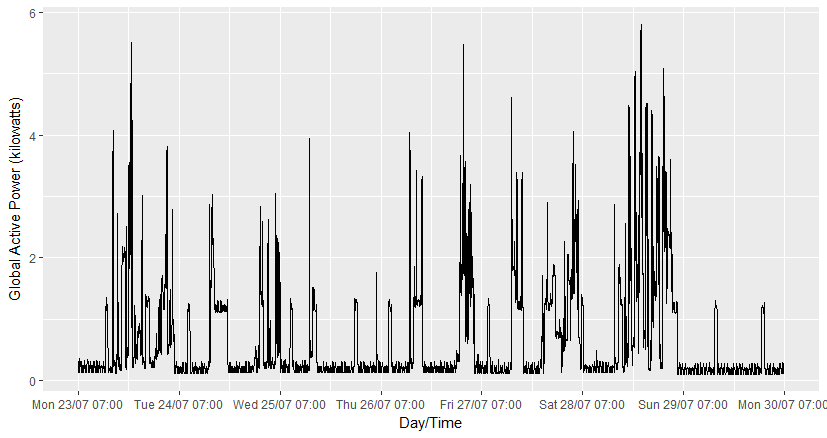
\includegraphics[scale=0.5]{fig1}
  \caption{Global active power in a week}
\end{figure}
In Figure 2, we can see that power usage increases in the morning and evening of weekdays. We can also observe that it is higher on the weekends that on weekdays, with Sunday having the highest power consumption out of all the days of the week.
\begin{figure}[H]
  \centering
  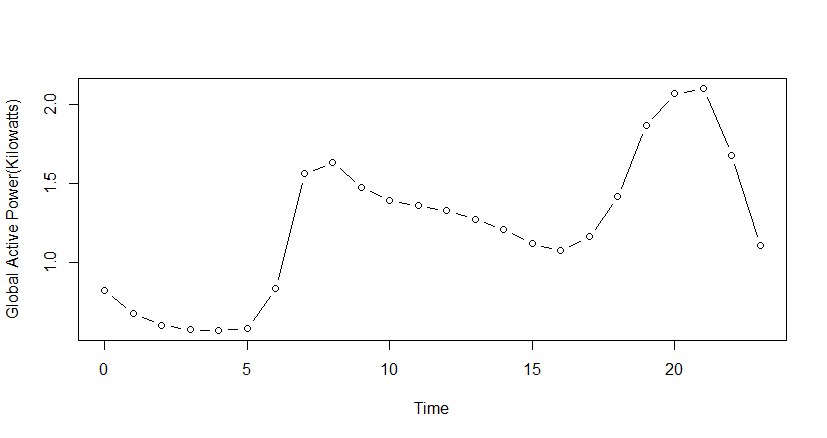
\includegraphics[scale=0.4]{fig2}
  \caption{Global active power in 24 hours}
\end{figure}
Moreover, in Figure 3, we can observe that at night time (from 12 AM to 5 AM), power consumption is close to zero. It begins to increase around 6 AM reaching a peak around 9 AM. It remains relatively stable throughout the afternoon, but later reaches another peak around 7-8 PM which could be attributed to family members coming back from work or school and settling down for the day. Based on these observations, we can guess that in the average household, family members wake up at 6 AM and go to bed at about 10 PM.
\begin{figure}[H]
  \centering
  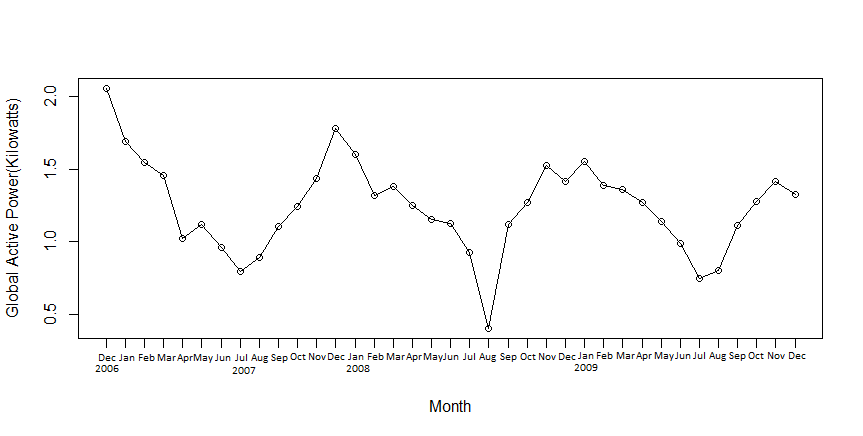
\includegraphics[scale=0.4]{fig3}
  \caption{Global active power every month}
\end{figure}
Additionally, in Figure 4, we can see an obvious trend that electricity usage reaches its peak at the start and end of every year, and goes to its lowest values in the middle of the year (from June to August). Therefore, we can infer that winter time in this location is probably from November to January, since cold temperature means that households use extra power to keep warm; and that summer time is between June and August, which corresponds to higher temperature and less electricity consumption.
\begin{figure}[H]
  \centering
  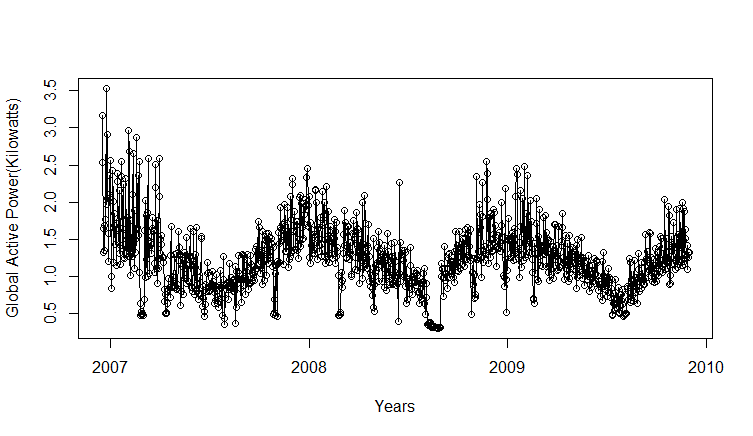
\includegraphics[scale=0.4]{fig4}
  \caption{Global active power every year}
\end{figure}
Moreover, when comparing the level and density of power consumption in every year interval (Figure 5), we can see that the usage of electricity has been decreasing. We can guess that their electricity use have become more economical or that the number of people in the household may have reduced.
\begin{figure}[H]
  \centering
  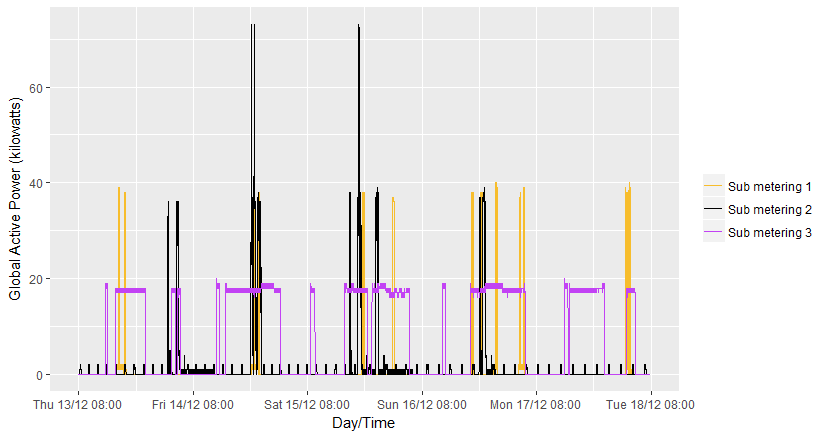
\includegraphics[scale=0.4]{fig5}
  \caption{Global active power in sub metering}
\end{figure}
Also, the datasets include measurements about specific electric appliances in the household. As described previously, sub metering 1 corresponds to the kitchen appliances, sub metering 2 corresponds to the laundry room, and sub metering 3 corresponds to heater and air-conditioner. Based on Figure 6, we can observe that kitchen electricity usage is low everyday in the morning and high everyday in the evening. The electricity usage of the laundry room is low on weekdays, and increases toward the end of the week. Becoming higher on Fridays and Mondays, and highest on Saturdays and Sundays. Electricity usage due to heating and air-conditioning is low in the mornings and high in the evenings.

\section{Experimental Analysis}
\subsection{Overview}
The experiments for this paper consisted of testing both univariate and multivariate Hidden Markov Models with a varying number of states in an attempt to find a model that would best represent the given datasets. In addition, experiments were performed with noise added to part of the non-anomalous training dataset (validation set) in order to obtain a quantitative measure of the accuracy of the trained models. Finally, after training the models, they were used to search the datasets for both point anomalies and collective anomalies.

\subsection{Process}
As explained previously, various preprocessing steps were performed on the data before using it to train and test the models. Some of this preprocessing involved splitting the training dataset into two parts: the first contained 90\% of the data points and would be used as training data to create the actual model while the second part contained the remaining 10\% and was used as the validation data to provide a way to measure how well the model fitted the dataset.

Once the data has been partitioned, the next step is to set up the parameters for training the Markov model. Once an arbitrary number of hidden states is chosen, the initial parameters for the transition matrix must be specified. For these experiments, it was decided to use the naive approach of setting the probability of transitioning from the current state to any other state, to equal values (uniformly distributed). These probabilities will be updated later when the HMM is fitted and the specification is created by means of the Viterbi algorithm. Next, the initial output probabilities must be defined by providing a Gaussian distribution consisting of the means and standard deviations for the states. Do to so, an approach using K-means clustering was chosen. K-means clustering is a method of clustering \textit{n} data points into \textit{k} clusters such that a data point is grouped into the cluster with a mean value that is closest it's value. Once the points have all been assigned to a cluster, the mean of each cluster is known, and the standard deviations can be computed, before passing both into the output probability matrix. The last required piece of information needed is the initial or starting state, for which a uniform distribution was used. With all of the required information specified, it is passed to the \textit{hmmspec()} function provided by the \textit{mhsmm} R library to create the model's specification. The final step in creating the model is to take the specification returned by the \textit{hmmspec()} function, and pass it to the \textit{hmmfit()} function to compute the probabilities.

With the model successfully trained, the experiments using it were performed. The first experiment was to use the validation data from earlier to test the accuracy of the model. Experiments using the validation data were performed first with the clean, unmodified validation data, and then after adding random noise to the data to simulate anomalous data, to ensure the model was accurately detecting anomalies.

To start off with, a univariate HMM was used, which used Global Active Power as it's sole variable. Experiments were run against this model using two, three, and four hidden states to find collective and point anomalies. Next, a multivariate HMM was used, using Global Active Power, Global Reactive Power, Voltage, And Global Intensity as the variables. These variables were chosen as there were shown to have a degree of correlation to each other. As with the univariate model, we used the multivariate model to find point and collective anomalies with two, three, and four states.

\section{Experimental Results}
The \textit{mhsmm} package calculates the log likelihood of generated models after the fitting is done. Log Likelihood is a tool for summarizing the data's evidence about unknown parameters\cite{log}. In the case of HMMs, it specifies how likely it is to observe a sequence like the training data, given the model that was constructed. Ideally we would like to obtain a negative log likelihood that is as close as possible to zero. The results obtained would suggest that out of the univariate HMMs, the one that most closely resembles the data is the one with four states. This model did provide ``good'' results in the detection of both point anomalies and collective anomalies, but it incurs in some degree of overfitting given the results that were obtained. Overfitting means that it tries to model the training set so closely that it later incurs in errors when predicting in the testing sets and possibly the validation set.

At the other end of the spectrum it the Univariate HMM with two states in which we can see a phenomenon called underfitting. This is in complete opposition to overfitting, since in this case the model is unable to capture the underlying trend or behavior of the system. This means that this model could potentially detect more anomalies than there really are.

In the case of multivariate HMMs we see the same pattern that was found in the univariate HMMs. The model that uses two states possibly suffers from some degree of underfitting and the model that uses four states possibly suffers from some degree of overfitting.

Out of the two models we had left (univariate HMM with three states and multivariate HMM with three states), we found that the univariate HMM provided the best fit to the system. This went against our initial expectations, since we assumed that the multivariate HMM would provide better accuracy given that it takes into consideration other variables of the dataset (Global reactive power, Voltage, Global intensity) which provide the model with more context information. We believe this happened because the anomaly detection method specified only takes into consideration the Global Active power. This gave the edge to the univariate HMM with 3 states, which the experimental results in figures 8 through 11 express.

\begin{figure}[H]
  \centering
  \footnotesize
  \resizebox{10cm}{!}{
  \begin{tabular}{|c|c|c|} \hline
    & \multicolumn{2}{|c|}{Log Likelihood (train data)} \\ \hline
    States & Univariate HMM & Multivariate HMM \\ \hline
    2 & -926607.9 & -5292092 \\ \hline
    3 & -566751.50 & -4693582 \\ \hline
    4 & -419092.2 & -4149228 \\ \hline
  \end{tabular}
  }
  \caption{Log Likelihood of train data}
\end{figure}
\begin{figure}[H]
  \centering
  \resizebox{10cm}{!}{
  \footnotesize
  \begin{tabular}{|c|c|c|c|c|c|c|c|} \hline
    \ & & \multicolumn{6}{|c|}{Threshold} \\ \hline
    \ & States & 0.50 & 1.00 & 1.25 & 1.50 & 1.75 & 2.00 \\ \hline
    \multirow{3}{*}{Univariate HMM} & 2 & 59064 & 31048 & 23239 & 17031 & 11585 & 9246 \\ \cline{2-8}
    & 3 & 43713 & 20852 & 15572 & 12169 & 9594 & 8213 \\ \cline{2-8}
    & 4 & 39448 & 19581 & 15632 & 12573 & 10222 & 8711 \\ \hline
    \multirow{3}{*}{Multivariate HMM} & 2 & 57438 & 34935 & 24086 & 16903 & 14571 & 12960 \\ \cline{2-8}
    & 3 & 57858 & 29482 & 23066 & 19166 & 14309 & 10790 \\ \cline{2-8}
    & 4 & 54919 & 30045 & 23262 & 19491 & 16167 & 12532 \\ \hline
  \end{tabular}
  }
  \caption{Point anomalies with noise}

  \resizebox{10cm}{!}{
  \begin{tabular}{|c|c|c|c|c|c|} \hline
    \ & & \multicolumn{4}{|c|}{Window Size} \\ \hline
    \ & States & 5 & 10 & 15 & 20 \\ \hline
    \multirow{3}{*}{Univariate HMM} & 2 & 14339 & 6503 & 4743 & 3433 \\ \cline{2-6}
    & 3 & 10307 & 5149 & 4061 & 2958 \\ \cline{2-6}
    & 4 & 10520 & 5240 & 4028 & 3006 \\ \hline
    \multirow{3}{*}{Multivariate HMM} & 2 & 14266 & 7101 & 4913 & 3578 \\ \cline{2-6}
    & 3 & 12835 & 6174 & 4046 & 3331 \\ \cline{2-6}
    & 4 & 13046 & 6267 & 4595 & 3374 \\ \hline
  \end{tabular}
  }
  \caption{Collective anomalies with noise}
\end{figure}
\begin{figure}[H]
  \centering
  \resizebox{10cm}{!}{
  \footnotesize
  \begin{tabular}{|c|c|c|c|c|c|c|c|} \hline
    \ & & \multicolumn{6}{|c|}{Threshold} \\ \hline
    \ & States & 0.50 & 1.00 & 1.25 & 1.50 & 1.75 & 2.00 \\ \hline
    \multirow{3}{*}{Univariate HMM} & 2 & 279461 & 169086 & 128317 & 81922 & 43597 & 29992 \\ \cline{2-8}
    & 3 & 224155 & 109478 & 71283 & 46447 & 29838 & 22857 \\ \cline{2-8}
    & 4 & 229259 & 113768 & 81357 & 55863 & 38301 & 29090 \\ \hline
    \multirow{3}{*}{Multivariate HMM} & 2 & 225391 & 106804 & 71287 & 40329 & 21574 & 14893 \\ \cline{2-8}
    & 3 & 209873 & 96408 & 58342 & 37317 & 23151 & 11659 \\ \cline{2-8}
    & 4 & 214104 & 85758 & 52617 & 32974 & 19280 & 10564 \\ \hline
  \end{tabular}
  }
  \caption{Point anomalies (test1.txt)}

  \resizebox{10cm}{!}{
  \begin{tabular}{|c|c|c|c|c|c|} \hline
    \ & & \multicolumn{4}{|c|}{Window Size} \\ \hline
    \ & States & 5 & 10 & 15 & 20 \\ \hline
    \multirow{3}{*}{Univariate HMM} & 2 & 29725 & 10609 & 7609 & 4499 \\ \cline{2-6}
    & 3 & 15646 & 4825 & 3387 & 1758 \\ \cline{2-6}
    & 4 & 17232 & 5089 & 3445 & 1746 \\ \hline
    \multirow{3}{*}{Multivariate HMM} & 2 & 14764 & 4694 & 3259 & 1960 \\ \cline{2-6}
    & 3 & 11449 & 3205 & 2186 & 1211 \\ \cline{2-6}
    & 4 & 8666 & 2512 & 1784 & 1023 \\ \hline
  \end{tabular}
  }
  \caption{Collective anomalies (test1.txt)}
\end{figure}

\section{Discussion}
One significant problem that was encountered in creating the experiments for this report was determining how to detect whether a data point was an anomaly or not. Initially, the idea was to compare against the standard deviation of the emission matrix, the thinking being that if the point falls outside of at most three standard deviations (99\% confidence interval) from the mean, it would likely be anomalous. Unfortunately, this method proved ineffective as it led to detecting large quantities of anomalies, up to 66\%, in the validation data before any noise was even added. In the end, a set threshold ranging from 0.5 to 2.0 was used for comparisons instead. Another problem we faced was determining what values to use for the initial state of the HMM for the transition and emission matrices, as well as the initial state of the model. There are many different takes on this problem, but ultimately it was decided to use K-means clustering for the emission matrix and use naive approaches for the transition matrix (equal weighting to all probabilities) and initial state.

If these experiments were to be taken further, there are a few ideas that could be pursued. The first is to implement an HSMM instead of an HMM. Since an HSMM takes the amount of time spent in a state into account when deciding if a transition should occur, it would be a good fit for power grid data where the usage is often consistently high at certain points of the day, and low at others. Secondly, using variables other than using only the Global Active Power in the univariate HMM to detect anomalies would be worth investigating to see if there are potential signs of intrusion based on those other variables. Finally, multivariate HMMs using different combinations of variables could be explored as there may be unseen correlation between the variables that were glossed over in the initial experiments.

\section{Conclusion}
Overall, a lot was learned about anomaly detection, Markov models, and statistical tools. Through this project, a greater understanding of how hidden Markov models work was gained and gave insight into how useful they could be in the future of cyber security. There is a lot of potential in using Markov models for this type of anomaly detection work, and as it is iterated over time by many other people, it could become a vital tool in the ongoing battle against cyber attacks towards critical infrastructure worldwide.

\section{Contribution of Group Members}
Matheson: Introduction, Background, Discussion, Conclusion, Experimental Analysis, helped develop algorithms\\ Alexis: Experiment Results, coded majority of R scripts  \\ Truong: Methodology, graphs and R scripts to generate them

\newpage
\bibliographystyle{abbrv}
\bibliography{report}


\end{document}
